% Created 2021-11-23 Tue 09:24
% Intended LaTeX compiler: pdflatex
\documentclass[11pt]{article}
\usepackage[utf8]{inputenc}
\usepackage[T1]{fontenc}
\usepackage{graphicx}
\usepackage{longtable}
\usepackage{wrapfig}
\usepackage{rotating}
\usepackage[normalem]{ulem}
\usepackage{amsmath}
\usepackage{amssymb}
\usepackage{capt-of}
\usepackage{hyperref}
\graphicspath{{../../books/}}
% wrong resolution of image
% https://tex.stackexchange.com/questions/21627/image-from-includegraphics-showing-in-wrong-image-size?rq=1

%%%%%%%%%%%%%%%%%%%%%%%%%%%%%%%%%%%%%%
%% TIPS                                 %%
%%%%%%%%%%%%%%%%%%%%%%%%%%%%%%%%%%%%%%
% \substack{a\\b} for multiple lines text
% \usepackage{expl3}
% \expandafter\def\csname ver@l3regex.sty\endcsname{}
% \usepackage{pkgloader}
\usepackage[utf8]{inputenc}

% nfss error
% \usepackage[B1,T1]{fontenc}
\usepackage{fontspec}

% \usepackage[Emoticons]{ucharclasses}
\newfontfamily\DejaSans{DejaVu Sans}
% \setDefaultTransitions{\DejaSans}{}

% pdfplots will load xolor automatically without option
\usepackage[dvipsnames]{xcolor}

%                                                             ┳┳┓   ┓
%                                                             ┃┃┃┏┓╋┣┓
%                                                             ┛ ┗┗┻┗┛┗
% \usepackage{amsmath} mathtools loads the amsmath
\usepackage{amsmath}
\usepackage{mathtools}

\usepackage{amsthm}
\usepackage{amsbsy}

%\usepackage{commath}

\usepackage{amssymb}

\usepackage{mathrsfs}
%\usepackage{mathabx}
\usepackage{stmaryrd}
\usepackage{empheq}

\usepackage{scalerel}
\usepackage{stackengine}
\usepackage{stackrel}



\usepackage{nicematrix}
\usepackage{tensor}
\usepackage{blkarray}
\usepackage{siunitx}
\usepackage[f]{esvect}

% centering \not on a letter
\usepackage{slashed}
\usepackage[makeroom]{cancel}

%\usepackage{merriweather}
\usepackage{unicode-math}
\setmainfont{TeX Gyre Pagella}
% \setmathfont{STIX}
%\setmathfont{texgyrepagella-math.otf}
%\setmathfont{Libertinus Math}
\setmathfont{Latin Modern Math}

 % \setmathfont[range={\smwhtdiamond,\enclosediamond,\varlrtriangle}]{Latin Modern Math}
\setmathfont[range={\rightrightarrows,\twoheadrightarrow,\leftrightsquigarrow,\triangledown,\vartriangle,\precneq,\succneq,\prec,\succ,\preceq,\succeq,\tieconcat}]{XITS Math}
 \setmathfont[range={\int,\setminus}]{Libertinus Math}
 % \setmathfont[range={\mathalpha}]{TeX Gyre Pagella Math}
%\setmathfont[range={\mitA,\mitB,\mitC,\mitD,\mitE,\mitF,\mitG,\mitH,\mitI,\mitJ,\mitK,\mitL,\mitM,\mitN,\mitO,\mitP,\mitQ,\mitR,\mitS,\mitT,\mitU,\mitV,\mitW,\mitX,\mitY,\mitZ,\mita,\mitb,\mitc,\mitd,\mite,\mitf,\mitg,\miti,\mitj,\mitk,\mitl,\mitm,\mitn,\mito,\mitp,\mitq,\mitr,\mits,\mitt,\mitu,\mitv,\mitw,\mitx,\mity,\mitz}]{TeX Gyre Pagella Math}
% unicode is not good at this!
%\let\nmodels\nvDash

 \usepackage{wasysym}

 % for wide hat
 \DeclareSymbolFont{yhlargesymbols}{OMX}{yhex}{m}{n} \DeclareMathAccent{\what}{\mathord}{yhlargesymbols}{"62}

%                                                               ┏┳┓•┓
%                                                                ┃ ┓┃┏┓
%                                                                ┻ ┗┛┗┗

\usepackage{pgfplots}
\pgfplotsset{compat=1.18}
\usepackage{tikz}
\usepackage{tikz-cd}
\tikzcdset{scale cd/.style={every label/.append style={scale=#1},
    cells={nodes={scale=#1}}}}
% TODO: discard qtree and use forest
% \usepackage{tikz-qtree}
\usepackage{forest}

\usetikzlibrary{arrows,positioning,calc,fadings,decorations,matrix,decorations,shapes.misc}
%setting from geogebra
\definecolor{ccqqqq}{rgb}{0.8,0,0}

%                                                          ┳┳┓•    ┓┓
%                                                          ┃┃┃┓┏┏┏┓┃┃┏┓┏┓┏┓┏┓┓┏┏
%                                                          ┛ ┗┗┛┗┗ ┗┗┗┻┛┗┗ ┗┛┗┻┛
%\usepackage{twemojis}
\usepackage[most]{tcolorbox}
\usepackage{threeparttable}
\usepackage{tabularx}

\usepackage{enumitem}
\usepackage[indLines=false]{algpseudocodex}
\usepackage[]{algorithm2e}
% \SetKwComment{Comment}{/* }{ */}
% \algrenewcommand\algorithmicrequire{\textbf{Input:}}
% \algrenewcommand\algorithmicensure{\textbf{Output:}}
% wrong with preview
\usepackage{subcaption}
\usepackage{caption}
% {\aunclfamily\Huge}
\usepackage{auncial}

\usepackage{float}

\usepackage{fancyhdr}

\usepackage{ifthen}
\usepackage{xargs}

\definecolor{mintedbg}{rgb}{0.99,0.99,0.99}
\usepackage[cachedir=\detokenize{~/miscellaneous/trash}]{minted}
\setminted{breaklines,
  mathescape,
  bgcolor=mintedbg,
  fontsize=\footnotesize,
  frame=single,
  linenos}
\usemintedstyle{xcode}
\usepackage{tcolorbox}
\usepackage{etoolbox}



\usepackage{imakeidx}
\usepackage{hyperref}
\usepackage{soul}
\usepackage{framed}

% don't use this for preview
%\usepackage[margin=1.5in]{geometry}
% \usepackage{geometry}
% \geometry{legalpaper, landscape, margin=1in}
\usepackage[font=itshape]{quoting}

%\LoadPackagesNow
%\usepackage[xetex]{preview}
%%%%%%%%%%%%%%%%%%%%%%%%%%%%%%%%%%%%%%%
%% USEPACKAGES end                       %%
%%%%%%%%%%%%%%%%%%%%%%%%%%%%%%%%%%%%%%%

%%%%%%%%%%%%%%%%%%%%%%%%%%%%%%%%%%%%%%%
%% Algorithm environment
%%%%%%%%%%%%%%%%%%%%%%%%%%%%%%%%%%%%%%%
\SetKwIF{Recv}{}{}{upon receiving}{do}{}{}{}
\SetKwBlock{Init}{initially do}{}
\SetKwProg{Function}{Function}{:}{}

% https://github.com/chrmatt/algpseudocodex/issues/3
\algnewcommand\algorithmicswitch{\textbf{switch}}%
\algnewcommand\algorithmiccase{\textbf{case}}
\algnewcommand\algorithmicof{\textbf{of}}
\algnewcommand\algorithmicotherwise{\texttt{otherwise} $\Rightarrow$}

\makeatletter
\algdef{SE}[SWITCH]{Switch}{EndSwitch}[1]{\algpx@startIndent\algpx@startCodeCommand\algorithmicswitch\ #1\ \algorithmicdo}{\algpx@endIndent\algpx@startCodeCommand\algorithmicend\ \algorithmicswitch}%
\algdef{SE}[CASE]{Case}{EndCase}[1]{\algpx@startIndent\algpx@startCodeCommand\algorithmiccase\ #1}{\algpx@endIndent\algpx@startCodeCommand\algorithmicend\ \algorithmiccase}%
\algdef{SE}[CASEOF]{CaseOf}{EndCaseOf}[1]{\algpx@startIndent\algpx@startCodeCommand\algorithmiccase\ #1 \algorithmicof}{\algpx@endIndent\algpx@startCodeCommand\algorithmicend\ \algorithmiccase}
\algdef{SE}[OTHERWISE]{Otherwise}{EndOtherwise}[0]{\algpx@startIndent\algpx@startCodeCommand\algorithmicotherwise}{\algpx@endIndent\algpx@startCodeCommand\algorithmicend\ \algorithmicotherwise}
\ifbool{algpx@noEnd}{%
  \algtext*{EndSwitch}%
  \algtext*{EndCase}%
  \algtext*{EndCaseOf}
  \algtext*{EndOtherwise}
  %
  % end indent line after (not before), to get correct y position for multiline text in last command
  \apptocmd{\EndSwitch}{\algpx@endIndent}{}{}%
  \apptocmd{\EndCase}{\algpx@endIndent}{}{}%
  \apptocmd{\EndCaseOf}{\algpx@endIndent}{}{}
  \apptocmd{\EndOtherwise}{\algpx@endIndent}{}{}
}{}%

\pretocmd{\Switch}{\algpx@endCodeCommand}{}{}
\pretocmd{\Case}{\algpx@endCodeCommand}{}{}
\pretocmd{\CaseOf}{\algpx@endCodeCommand}{}{}
\pretocmd{\Otherwise}{\algpx@endCodeCommand}{}{}

% for end commands that may not be printed, tell endCodeCommand whether we are using noEnd
\ifbool{algpx@noEnd}{%
  \pretocmd{\EndSwitch}{\algpx@endCodeCommand[1]}{}{}%
  \pretocmd{\EndCase}{\algpx@endCodeCommand[1]}{}{}
  \pretocmd{\EndCaseOf}{\algpx@endCodeCommand[1]}{}{}%
  \pretocmd{\EndOtherwise}{\algpx@endCodeCommand[1]}{}{}
}{%
  \pretocmd{\EndSwitch}{\algpx@endCodeCommand[0]}{}{}%
  \pretocmd{\EndCase}{\algpx@endCodeCommand[0]}{}{}%
  \pretocmd{\EndCaseOf}{\algpx@endCodeCommand[0]}{}{}
  \pretocmd{\EndOtherwise}{\algpx@endCodeCommand[0]}{}{}
}%
\makeatother
% % For algpseudocode
% \algnewcommand\algorithmicswitch{\textbf{switch}}
% \algnewcommand\algorithmiccase{\textbf{case}}
% \algnewcommand\algorithmiccaseof{\textbf{case}}
% \algnewcommand\algorithmicof{\textbf{of}}
% % New "environments"
% \algdef{SE}[SWITCH]{Switch}{EndSwitch}[1]{\algorithmicswitch\ #1\ \algorithmicdo}{\algorithmicend\ \algorithmicswitch}%
% \algdef{SE}[CASE]{Case}{EndCase}[1]{\algorithmiccase\ #1}{\algorithmicend\ \algorithmiccase}%
% \algtext*{EndSwitch}%
% \algtext*{EndCase}
% \algdef{SE}[CASEOF]{CaseOf}{EndCaseOf}[1]{\algorithmiccaseof\ #1 \algorithmicof}{\algorithmicend\ \algorithmiccaseof}
% \algtext*{EndCaseOf}



%\pdfcompresslevel0

% quoting from
% https://tex.stackexchange.com/questions/391726/the-quotation-environment
\NewDocumentCommand{\bywhom}{m}{% the Bourbaki trick
  {\nobreak\hfill\penalty50\hskip1em\null\nobreak
   \hfill\mbox{\normalfont(#1)}%
   \parfillskip=0pt \finalhyphendemerits=0 \par}%
}

\NewDocumentEnvironment{pquotation}{m}
  {\begin{quoting}[
     indentfirst=true,
     leftmargin=\parindent,
     rightmargin=\parindent]\itshape}
  {\bywhom{#1}\end{quoting}}

\indexsetup{othercode=\small}
\makeindex[columns=2,options={-s /media/wu/file/stuuudy/notes/index_style.ist},intoc]
\makeatletter
\def\@idxitem{\par\hangindent 0pt}
\makeatother


% \newcounter{dummy} \numberwithin{dummy}{section}
\newtheorem{dummy}{dummy}[section]
\theoremstyle{definition}
\newtheorem{definition}[dummy]{Definition}
\theoremstyle{plain}
\newtheorem{corollary}[dummy]{Corollary}
\newtheorem{lemma}[dummy]{Lemma}
\newtheorem{proposition}[dummy]{Proposition}
\newtheorem{theorem}[dummy]{Theorem}
\newtheorem{notation}[dummy]{Notation}
\newtheorem{conjecture}[dummy]{Conjecture}
\newtheorem{fact}[dummy]{Fact}
\newtheorem{warning}[dummy]{Warning}
\theoremstyle{definition}
\newtheorem{examplle}{Example}[section]
\theoremstyle{remark}
\newtheorem*{remark}{Remark}
\newtheorem{exercise}{Exercise}[subsection]
\newtheorem{problem}{Problem}[subsection]
\newtheorem{observation}{Observation}[section]
\newenvironment{claim}[1]{\par\noindent\textbf{Claim:}\space#1}{}

\makeatletter
\DeclareFontFamily{U}{tipa}{}
\DeclareFontShape{U}{tipa}{m}{n}{<->tipa10}{}
\newcommand{\arc@char}{{\usefont{U}{tipa}{m}{n}\symbol{62}}}%

\newcommand{\arc}[1]{\mathpalette\arc@arc{#1}}

\newcommand{\arc@arc}[2]{%
  \sbox0{$\m@th#1#2$}%
  \vbox{
    \hbox{\resizebox{\wd0}{\height}{\arc@char}}
    \nointerlineskip
    \box0
  }%
}
\makeatother

\setcounter{MaxMatrixCols}{20}
%%%%%%% ABS
\DeclarePairedDelimiter\abss{\lvert}{\rvert}%
\DeclarePairedDelimiter\normm{\lVert}{\rVert}%

% Swap the definition of \abs* and \norm*, so that \abs
% and \norm resizes the size of the brackets, and the
% starred version does not.
\makeatletter
\let\oldabs\abss
%\def\abs{\@ifstar{\oldabs}{\oldabs*}}
\newcommand{\abs}{\@ifstar{\oldabs}{\oldabs*}}
\newcommand{\norm}[1]{\left\lVert#1\right\rVert}
%\let\oldnorm\normm
%\def\norm{\@ifstar{\oldnorm}{\oldnorm*}}
%\renewcommand{norm}{\@ifstar{\oldnorm}{\oldnorm*}}
\makeatother

% \stackMath
% \newcommand\what[1]{%
% \savestack{\tmpbox}{\stretchto{%
%   \scaleto{%
%     \scalerel*[\widthof{\ensuremath{#1}}]{\kern-.6pt\bigwedge\kern-.6pt}%
%     {\rule[-\textheight/2]{1ex}{\textheight}}%WIDTH-LIMITED BIG WEDGE
%   }{\textheight}%
% }{0.5ex}}%
% \stackon[1pt]{#1}{\tmpbox}%
% }

% \newcommand\what[1]{\ThisStyle{%
%     \setbox0=\hbox{$\SavedStyle#1$}%
%     \stackengine{-1.0\ht0+.5pt}{$\SavedStyle#1$}{%
%       \stretchto{\scaleto{\SavedStyle\mkern.15mu\char'136}{2.6\wd0}}{1.4\ht0}%
%     }{O}{c}{F}{T}{S}%
%   }
% }

% \newcommand\wtilde[1]{\ThisStyle{%
%     \setbox0=\hbox{$\SavedStyle#1$}%
%     \stackengine{-.1\LMpt}{$\SavedStyle#1$}{%
%       \stretchto{\scaleto{\SavedStyle\mkern.2mu\AC}{.5150\wd0}}{.6\ht0}%
%     }{O}{c}{F}{T}{S}%
%   }
% }

% \newcommand\wbar[1]{\ThisStyle{%
%     \setbox0=\hbox{$\SavedStyle#1$}%
%     \stackengine{.5pt+\LMpt}{$\SavedStyle#1$}{%
%       \rule{\wd0}{\dimexpr.3\LMpt+.3pt}%
%     }{O}{c}{F}{T}{S}%
%   }
% }

\newcommand{\bl}[1] {\boldsymbol{#1}}
\newcommand{\Wt}[1] {\stackrel{\sim}{\smash{#1}\rule{0pt}{1.1ex}}}
\newcommand{\wt}[1] {\widetilde{#1}}
\newcommand{\tf}[1] {\textbf{#1}}

\newcommand{\wu}[1]{{\color{red} #1}}

%For boxed texts in align, use Aboxed{}
%otherwise use boxed{}

\DeclareMathSymbol{\widehatsym}{\mathord}{largesymbols}{"62}
\newcommand\lowerwidehatsym{%
  \text{\smash{\raisebox{-1.3ex}{%
    $\widehatsym$}}}}
\newcommand\fixwidehat[1]{%
  \mathchoice
    {\accentset{\displaystyle\lowerwidehatsym}{#1}}
    {\accentset{\textstyle\lowerwidehatsym}{#1}}
    {\accentset{\scriptstyle\lowerwidehatsym}{#1}}
    {\accentset{\scriptscriptstyle\lowerwidehatsym}{#1}}
  }


\newcommand{\cupdot}{\mathbin{\dot{\cup}}}
\newcommand{\bigcupdot}{\mathop{\dot{\bigcup}}}

\usepackage{graphicx}

\usepackage[toc,page]{appendix}

% text on arrow for xRightarrow
\makeatletter
%\newcommand{\xRightarrow}[2][]{\ext@arrow 0359\Rightarrowfill@{#1}{#2}}
\makeatother

% Arbitrary long arrow
\newcommand{\Rarrow}[1]{%
\parbox{#1}{\tikz{\draw[->](0,0)--(#1,0);}}
}

\newcommand{\LRarrow}[1]{%
\parbox{#1}{\tikz{\draw[<->](0,0)--(#1,0);}}
}


\makeatletter
\providecommand*{\rmodels}{%
  \mathrel{%
    \mathpalette\@rmodels\models
  }%
}
\newcommand*{\@rmodels}[2]{%
  \reflectbox{$\m@th#1#2$}%
}
\makeatother

% Roman numerals
\makeatletter
\newcommand*{\rom}[1]{\expandafter\@slowromancap\romannumeral #1@}
\makeatother
% \\def \\b\([a-zA-Z]\) {\\boldsymbol{[a-zA-z]}}
% \\DeclareMathOperator{\\b\1}{\\textbf{\1}}

\DeclareMathOperator*{\argmin}{arg\,min}
\DeclareMathOperator*{\argmax}{arg\,max}

\DeclareMathOperator{\bone}{\textbf{1}}
\DeclareMathOperator{\bx}{\textbf{x}}
\DeclareMathOperator{\bz}{\textbf{z}}
\DeclareMathOperator{\bff}{\textbf{f}}
\DeclareMathOperator{\ba}{\textbf{a}}
\DeclareMathOperator{\bk}{\textbf{k}}
\DeclareMathOperator{\bs}{\textbf{s}}
\DeclareMathOperator{\bh}{\textbf{h}}
\DeclareMathOperator{\bc}{\textbf{c}}
\DeclareMathOperator{\br}{\textbf{r}}
\DeclareMathOperator{\bi}{\textbf{i}}
\DeclareMathOperator{\bj}{\textbf{j}}
\DeclareMathOperator{\bn}{\textbf{n}}
\DeclareMathOperator{\be}{\textbf{e}}
\DeclareMathOperator{\bo}{\textbf{o}}
\DeclareMathOperator{\bU}{\textbf{U}}
\DeclareMathOperator{\bL}{\textbf{L}}
\DeclareMathOperator{\bV}{\textbf{V}}
\def \bzero {\mathbf{0}}
\def \bbone {\mathbb{1}}
\def \btwo {\mathbf{2}}
\DeclareMathOperator{\bv}{\textbf{v}}
\DeclareMathOperator{\bp}{\textbf{p}}
\DeclareMathOperator{\bI}{\textbf{I}}
\def \dbI {\dot{\bI}}
\DeclareMathOperator{\bM}{\textbf{M}}
\DeclareMathOperator{\bN}{\textbf{N}}
\DeclareMathOperator{\bK}{\textbf{K}}
\DeclareMathOperator{\bt}{\textbf{t}}
\DeclareMathOperator{\bb}{\textbf{b}}
\DeclareMathOperator{\bA}{\textbf{A}}
\DeclareMathOperator{\bX}{\textbf{X}}
\DeclareMathOperator{\bu}{\textbf{u}}
\DeclareMathOperator{\bS}{\textbf{S}}
\DeclareMathOperator{\bZ}{\textbf{Z}}
\DeclareMathOperator{\bJ}{\textbf{J}}
\DeclareMathOperator{\by}{\textbf{y}}
\DeclareMathOperator{\bw}{\textbf{w}}
\DeclareMathOperator{\bT}{\textbf{T}}
\DeclareMathOperator{\bF}{\textbf{F}}
\DeclareMathOperator{\bmm}{\textbf{m}}
\DeclareMathOperator{\bW}{\textbf{W}}
\DeclareMathOperator{\bR}{\textbf{R}}
\DeclareMathOperator{\bC}{\textbf{C}}
\DeclareMathOperator{\bD}{\textbf{D}}
\DeclareMathOperator{\bE}{\textbf{E}}
\DeclareMathOperator{\bQ}{\textbf{Q}}
\DeclareMathOperator{\bP}{\textbf{P}}
\DeclareMathOperator{\bY}{\textbf{Y}}
\DeclareMathOperator{\bH}{\textbf{H}}
\DeclareMathOperator{\bB}{\textbf{B}}
\DeclareMathOperator{\bG}{\textbf{G}}
\def \blambda {\symbf{\lambda}}
\def \boldeta {\symbf{\eta}}
\def \balpha {\symbf{\alpha}}
\def \btau {\symbf{\tau}}
\def \bbeta {\symbf{\beta}}
\def \bgamma {\symbf{\gamma}}
\def \bxi {\symbf{\xi}}
\def \bLambda {\symbf{\Lambda}}
\def \bGamma {\symbf{\Gamma}}

\newcommand{\bto}{{\boldsymbol{\to}}}
\newcommand{\Ra}{\Rightarrow}
\newcommand{\xrsa}[1]{\overset{#1}{\rightsquigarrow}}
\newcommand{\xlsa}[1]{\overset{#1}{\leftsquigarrow}}
\newcommand\und[1]{\underline{#1}}
\newcommand\ove[1]{\overline{#1}}
%\def \concat {\verb|^|}
\def \bPhi {\mbfPhi}
\def \btheta {\mbftheta}
\def \bTheta {\mbfTheta}
\def \bmu {\mbfmu}
\def \bphi {\mbfphi}
\def \bSigma {\mbfSigma}
\def \la {\langle}
\def \ra {\rangle}

\def \caln {\mathcal{N}}
\def \dissum {\displaystyle\Sigma}
\def \dispro {\displaystyle\prod}

\def \caret {\verb!^!}

\def \A {\mathbb{A}}
\def \B {\mathbb{B}}
\def \C {\mathbb{C}}
\def \D {\mathbb{D}}
\def \E {\mathbb{E}}
\def \F {\mathbb{F}}
\def \G {\mathbb{G}}
\def \H {\mathbb{H}}
\def \I {\mathbb{I}}
\def \J {\mathbb{J}}
\def \K {\mathbb{K}}
\def \L {\mathbb{L}}
\def \M {\mathbb{M}}
\def \N {\mathbb{N}}
\def \O {\mathbb{O}}
\def \P {\mathbb{P}}
\def \Q {\mathbb{Q}}
\def \R {\mathbb{R}}
\def \S {\mathbb{S}}
\def \T {\mathbb{T}}
\def \U {\mathbb{U}}
\def \V {\mathbb{V}}
\def \W {\mathbb{W}}
\def \X {\mathbb{X}}
\def \Y {\mathbb{Y}}
\def \Z {\mathbb{Z}}

\def \cala {\mathcal{A}}
\def \cale {\mathcal{E}}
\def \calb {\mathcal{B}}
\def \calq {\mathcal{Q}}
\def \calp {\mathcal{P}}
\def \cals {\mathcal{S}}
\def \calx {\mathcal{X}}
\def \caly {\mathcal{Y}}
\def \calg {\mathcal{G}}
\def \cald {\mathcal{D}}
\def \caln {\mathcal{N}}
\def \calr {\mathcal{R}}
\def \calt {\mathcal{T}}
\def \calm {\mathcal{M}}
\def \calw {\mathcal{W}}
\def \calc {\mathcal{C}}
\def \calv {\mathcal{V}}
\def \calf {\mathcal{F}}
\def \calk {\mathcal{K}}
\def \call {\mathcal{L}}
\def \calu {\mathcal{U}}
\def \calo {\mathcal{O}}
\def \calh {\mathcal{H}}
\def \cali {\mathcal{I}}
\def \calj {\mathcal{J}}

\def \bcup {\bigcup}

% set theory

\def \zfcc {\textbf{ZFC}^-}
\def \BGC {\textbf{BGC}}
\def \BG {\textbf{BG}}
\def \ac  {\textbf{AC}}
\def \gl  {\textbf{L }}
\def \gll {\textbf{L}}
\newcommand{\zfm}{$\textbf{ZF}^-$}

\def \ZFm {\text{ZF}^-}
\def \ZFCm {\text{ZFC}^-}
\DeclareMathOperator{\WF}{WF}
\DeclareMathOperator{\On}{On}
\def \on {\textbf{On }}
\def \cm {\textbf{M }}
\def \cn {\textbf{N }}
\def \cv {\textbf{V }}
\def \zc {\textbf{ZC }}
\def \zcm {\textbf{ZC}}
\def \zff {\textbf{ZF}}
\def \wfm {\textbf{WF}}
\def \onm {\textbf{On}}
\def \cmm {\textbf{M}}
\def \cnm {\textbf{N}}
\def \cvm {\textbf{V}}

\renewcommand{\restriction}{\mathord{\upharpoonright}}
%% another restriction
\newcommand\restr[2]{{% we make the whole thing an ordinary symbol
  \left.\kern-\nulldelimiterspace % automatically resize the bar with \right
  #1 % the function
  \vphantom{\big|} % pretend it's a little taller at normal size
  \right|_{#2} % this is the delimiter
  }}

\def \pred {\text{pred}}

\def \rank {\text{rank}}
\def \Con {\text{Con}}
\def \deff {\text{Def}}


\def \uin {\underline{\in}}
\def \oin {\overline{\in}}
\def \uR {\underline{R}}
\def \oR {\overline{R}}
\def \uP {\underline{P}}
\def \oP {\overline{P}}

\def \dsum {\displaystyle\sum}

\def \Ra {\Rightarrow}

\def \e {\enspace}

\def \sgn {\operatorname{sgn}}
\def \gen {\operatorname{gen}}
\def \Hom {\operatorname{Hom}}
\def \hom {\operatorname{hom}}
\def \Sub {\operatorname{Sub}}

\def \supp {\operatorname{supp}}

\def \epiarrow {\twoheadarrow}
\def \monoarrow {\rightarrowtail}
\def \rrarrow {\rightrightarrows}

% \def \minus {\text{-}}
% \newcommand{\minus}{\scalebox{0.75}[1.0]{$-$}}
% \DeclareUnicodeCharacter{002D}{\minus}


\def \tril {\triangleleft}

\def \ISigma {\text{I}\Sigma}
\def \IDelta {\text{I}\Delta}
\def \IPi {\text{I}\Pi}
\def \ACF {\textsf{ACF}}
\def \pCF {\textit{p}\text{CF}}
\def \ACVF {\textsf{ACVF}}
\def \HLR {\textsf{HLR}}
\def \OAG {\textsf{OAG}}
\def \RCF {\textsf{RCF}}
\DeclareMathOperator{\GL}{GL}
\DeclareMathOperator{\PGL}{PGL}
\DeclareMathOperator{\SL}{SL}
\DeclareMathOperator{\Inv}{Inv}
\DeclareMathOperator{\res}{res}
\DeclareMathOperator{\Sym}{Sym}
%\DeclareMathOperator{\char}{char}
\def \equal {=}

\def \degree {\text{degree}}
\def \app {\text{App}}
\def \FV {\text{FV}}
\def \conv {\text{conv}}
\def \cont {\text{cont}}
\DeclareMathOperator{\cl}{\text{cl}}
\DeclareMathOperator{\trcl}{\text{trcl}}
\DeclareMathOperator{\sg}{sg}
\DeclareMathOperator{\trdeg}{trdeg}
\def \Ord {\text{Ord}}

\DeclareMathOperator{\cf}{cf}
\DeclareMathOperator{\zfc}{ZFC}

%\DeclareMathOperator{\Th}{Th}
%\def \th {\text{Th}}
% \newcommand{\th}{\text{Th}}
\DeclareMathOperator{\type}{type}
\DeclareMathOperator{\zf}{\textbf{ZF}}
\def \fa {\mathfrak{a}}
\def \fb {\mathfrak{b}}
\def \fc {\mathfrak{c}}
\def \fd {\mathfrak{d}}
\def \fe {\mathfrak{e}}
\def \ff {\mathfrak{f}}
\def \fg {\mathfrak{g}}
\def \fh {\mathfrak{h}}
%\def \fi {\mathfrak{i}}
\def \fj {\mathfrak{j}}
\def \fk {\mathfrak{k}}
\def \fl {\mathfrak{l}}
\def \fm {\mathfrak{m}}
\def \fn {\mathfrak{n}}
\def \fo {\mathfrak{o}}
\def \fp {\mathfrak{p}}
\def \fq {\mathfrak{q}}
\def \fr {\mathfrak{r}}
\def \fs {\mathfrak{s}}
\def \ft {\mathfrak{t}}
\def \fu {\mathfrak{u}}
\def \fv {\mathfrak{v}}
\def \fw {\mathfrak{w}}
\def \fx {\mathfrak{x}}
\def \fy {\mathfrak{y}}
\def \fz {\mathfrak{z}}
\def \fA {\mathfrak{A}}
\def \fB {\mathfrak{B}}
\def \fC {\mathfrak{C}}
\def \fD {\mathfrak{D}}
\def \fE {\mathfrak{E}}
\def \fF {\mathfrak{F}}
\def \fG {\mathfrak{G}}
\def \fH {\mathfrak{H}}
\def \fI {\mathfrak{I}}
\def \fJ {\mathfrak{J}}
\def \fK {\mathfrak{K}}
\def \fL {\mathfrak{L}}
\def \fM {\mathfrak{M}}
\def \fN {\mathfrak{N}}
\def \fO {\mathfrak{O}}
\def \fP {\mathfrak{P}}
\def \fQ {\mathfrak{Q}}
\def \fR {\mathfrak{R}}
\def \fS {\mathfrak{S}}
\def \fT {\mathfrak{T}}
\def \fU {\mathfrak{U}}
\def \fV {\mathfrak{V}}
\def \fW {\mathfrak{W}}
\def \fX {\mathfrak{X}}
\def \fY {\mathfrak{Y}}
\def \fZ {\mathfrak{Z}}

\def \sfA {\textsf{A}}
\def \sfB {\textsf{B}}
\def \sfC {\textsf{C}}
\def \sfD {\textsf{D}}
\def \sfE {\textsf{E}}
\def \sfF {\textsf{F}}
\def \sfG {\textsf{G}}
\def \sfH {\textsf{H}}
\def \sfI {\textsf{I}}
\def \sfJ {\textsf{J}}
\def \sfK {\textsf{K}}
\def \sfL {\textsf{L}}
\def \sfM {\textsf{M}}
\def \sfN {\textsf{N}}
\def \sfO {\textsf{O}}
\def \sfP {\textsf{P}}
\def \sfQ {\textsf{Q}}
\def \sfR {\textsf{R}}
\def \sfS {\textsf{S}}
\def \sfT {\textsf{T}}
\def \sfU {\textsf{U}}
\def \sfV {\textsf{V}}
\def \sfW {\textsf{W}}
\def \sfX {\textsf{X}}
\def \sfY {\textsf{Y}}
\def \sfZ {\textsf{Z}}
\def \sfa {\textsf{a}}
\def \sfb {\textsf{b}}
\def \sfc {\textsf{c}}
\def \sfd {\textsf{d}}
\def \sfe {\textsf{e}}
\def \sff {\textsf{f}}
\def \sfg {\textsf{g}}
\def \sfh {\textsf{h}}
\def \sfi {\textsf{i}}
\def \sfj {\textsf{j}}
\def \sfk {\textsf{k}}
\def \sfl {\textsf{l}}
\def \sfm {\textsf{m}}
\def \sfn {\textsf{n}}
\def \sfo {\textsf{o}}
\def \sfp {\textsf{p}}
\def \sfq {\textsf{q}}
\def \sfr {\textsf{r}}
\def \sfs {\textsf{s}}
\def \sft {\textsf{t}}
\def \sfu {\textsf{u}}
\def \sfv {\textsf{v}}
\def \sfw {\textsf{w}}
\def \sfx {\textsf{x}}
\def \sfy {\textsf{y}}
\def \sfz {\textsf{z}}

\def \ttA {\texttt{A}}
\def \ttB {\texttt{B}}
\def \ttC {\texttt{C}}
\def \ttD {\texttt{D}}
\def \ttE {\texttt{E}}
\def \ttF {\texttt{F}}
\def \ttG {\texttt{G}}
\def \ttH {\texttt{H}}
\def \ttI {\texttt{I}}
\def \ttJ {\texttt{J}}
\def \ttK {\texttt{K}}
\def \ttL {\texttt{L}}
\def \ttM {\texttt{M}}
\def \ttN {\texttt{N}}
\def \ttO {\texttt{O}}
\def \ttP {\texttt{P}}
\def \ttQ {\texttt{Q}}
\def \ttR {\texttt{R}}
\def \ttS {\texttt{S}}
\def \ttT {\texttt{T}}
\def \ttU {\texttt{U}}
\def \ttV {\texttt{V}}
\def \ttW {\texttt{W}}
\def \ttX {\texttt{X}}
\def \ttY {\texttt{Y}}
\def \ttZ {\texttt{Z}}
\def \tta {\texttt{a}}
\def \ttb {\texttt{b}}
\def \ttc {\texttt{c}}
\def \ttd {\texttt{d}}
\def \tte {\texttt{e}}
\def \ttf {\texttt{f}}
\def \ttg {\texttt{g}}
\def \tth {\texttt{h}}
\def \tti {\texttt{i}}
\def \ttj {\texttt{j}}
\def \ttk {\texttt{k}}
\def \ttl {\texttt{l}}
\def \ttm {\texttt{m}}
\def \ttn {\texttt{n}}
\def \tto {\texttt{o}}
\def \ttp {\texttt{p}}
\def \ttq {\texttt{q}}
\def \ttr {\texttt{r}}
\def \tts {\texttt{s}}
\def \ttt {\texttt{t}}
\def \ttu {\texttt{u}}
\def \ttv {\texttt{v}}
\def \ttw {\texttt{w}}
\def \ttx {\texttt{x}}
\def \tty {\texttt{y}}
\def \ttz {\texttt{z}}

\def \bara {\bbar{a}}
\def \barb {\bbar{b}}
\def \barc {\bbar{c}}
\def \bard {\bbar{d}}
\def \bare {\bbar{e}}
\def \barf {\bbar{f}}
\def \barg {\bbar{g}}
\def \barh {\bbar{h}}
\def \bari {\bbar{i}}
\def \barj {\bbar{j}}
\def \bark {\bbar{k}}
\def \barl {\bbar{l}}
\def \barm {\bbar{m}}
\def \barn {\bbar{n}}
\def \baro {\bbar{o}}
\def \barp {\bbar{p}}
\def \barq {\bbar{q}}
\def \barr {\bbar{r}}
\def \bars {\bbar{s}}
\def \bart {\bbar{t}}
\def \baru {\bbar{u}}
\def \barv {\bbar{v}}
\def \barw {\bbar{w}}
\def \barx {\bbar{x}}
\def \bary {\bbar{y}}
\def \barz {\bbar{z}}
\def \barA {\bbar{A}}
\def \barB {\bbar{B}}
\def \barC {\bbar{C}}
\def \barD {\bbar{D}}
\def \barE {\bbar{E}}
\def \barF {\bbar{F}}
\def \barG {\bbar{G}}
\def \barH {\bbar{H}}
\def \barI {\bbar{I}}
\def \barJ {\bbar{J}}
\def \barK {\bbar{K}}
\def \barL {\bbar{L}}
\def \barM {\bbar{M}}
\def \barN {\bbar{N}}
\def \barO {\bbar{O}}
\def \barP {\bbar{P}}
\def \barQ {\bbar{Q}}
\def \barR {\bbar{R}}
\def \barS {\bbar{S}}
\def \barT {\bbar{T}}
\def \barU {\bbar{U}}
\def \barVV {\bbar{V}}
\def \barW {\bbar{W}}
\def \barX {\bbar{X}}
\def \barY {\bbar{Y}}
\def \barZ {\bbar{Z}}

\def \baralpha {\bbar{\alpha}}
\def \bartau {\bbar{\tau}}
\def \barsigma {\bbar{\sigma}}
\def \barzeta {\bbar{\zeta}}

\def \hata {\hat{a}}
\def \hatb {\hat{b}}
\def \hatc {\hat{c}}
\def \hatd {\hat{d}}
\def \hate {\hat{e}}
\def \hatf {\hat{f}}
\def \hatg {\hat{g}}
\def \hath {\hat{h}}
\def \hati {\hat{i}}
\def \hatj {\hat{j}}
\def \hatk {\hat{k}}
\def \hatl {\hat{l}}
\def \hatm {\hat{m}}
\def \hatn {\hat{n}}
\def \hato {\hat{o}}
\def \hatp {\hat{p}}
\def \hatq {\hat{q}}
\def \hatr {\hat{r}}
\def \hats {\hat{s}}
\def \hatt {\hat{t}}
\def \hatu {\hat{u}}
\def \hatv {\hat{v}}
\def \hatw {\hat{w}}
\def \hatx {\hat{x}}
\def \haty {\hat{y}}
\def \hatz {\hat{z}}
\def \hatA {\hat{A}}
\def \hatB {\hat{B}}
\def \hatC {\hat{C}}
\def \hatD {\hat{D}}
\def \hatE {\hat{E}}
\def \hatF {\hat{F}}
\def \hatG {\hat{G}}
\def \hatH {\hat{H}}
\def \hatI {\hat{I}}
\def \hatJ {\hat{J}}
\def \hatK {\hat{K}}
\def \hatL {\hat{L}}
\def \hatM {\hat{M}}
\def \hatN {\hat{N}}
\def \hatO {\hat{O}}
\def \hatP {\hat{P}}
\def \hatQ {\hat{Q}}
\def \hatR {\hat{R}}
\def \hatS {\hat{S}}
\def \hatT {\hat{T}}
\def \hatU {\hat{U}}
\def \hatVV {\hat{V}}
\def \hatW {\hat{W}}
\def \hatX {\hat{X}}
\def \hatY {\hat{Y}}
\def \hatZ {\hat{Z}}

\def \hatphi {\hat{\phi}}

\def \barfM {\bbar{\fM}}
\def \barfN {\bbar{\fN}}

\def \tila {\tilde{a}}
\def \tilb {\tilde{b}}
\def \tilc {\tilde{c}}
\def \tild {\tilde{d}}
\def \tile {\tilde{e}}
\def \tilf {\tilde{f}}
\def \tilg {\tilde{g}}
\def \tilh {\tilde{h}}
\def \tili {\tilde{i}}
\def \tilj {\tilde{j}}
\def \tilk {\tilde{k}}
\def \till {\tilde{l}}
\def \tilm {\tilde{m}}
\def \tiln {\tilde{n}}
\def \tilo {\tilde{o}}
\def \tilp {\tilde{p}}
\def \tilq {\tilde{q}}
\def \tilr {\tilde{r}}
\def \tils {\tilde{s}}
\def \tilt {\tilde{t}}
\def \tilu {\tilde{u}}
\def \tilv {\tilde{v}}
\def \tilw {\tilde{w}}
\def \tilx {\tilde{x}}
\def \tily {\tilde{y}}
\def \tilz {\tilde{z}}
\def \tilA {\tilde{A}}
\def \tilB {\tilde{B}}
\def \tilC {\tilde{C}}
\def \tilD {\tilde{D}}
\def \tilE {\tilde{E}}
\def \tilF {\tilde{F}}
\def \tilG {\tilde{G}}
\def \tilH {\tilde{H}}
\def \tilI {\tilde{I}}
\def \tilJ {\tilde{J}}
\def \tilK {\tilde{K}}
\def \tilL {\tilde{L}}
\def \tilM {\tilde{M}}
\def \tilN {\tilde{N}}
\def \tilO {\tilde{O}}
\def \tilP {\tilde{P}}
\def \tilQ {\tilde{Q}}
\def \tilR {\tilde{R}}
\def \tilS {\tilde{S}}
\def \tilT {\tilde{T}}
\def \tilU {\tilde{U}}
\def \tilVV {\tilde{V}}
\def \tilW {\tilde{W}}
\def \tilX {\tilde{X}}
\def \tilY {\tilde{Y}}
\def \tilZ {\tilde{Z}}

\def \tilalpha {\tilde{\alpha}}
\def \tilPhi {\tilde{\Phi}}

\def \barnu {\bar{\nu}}
\def \barrho {\bar{\rho}}
%\DeclareMathOperator{\ker}{ker}
\DeclareMathOperator{\im}{im}

\DeclareMathOperator{\Inn}{Inn}
\DeclareMathOperator{\rel}{rel}
\def \dote {\stackrel{\cdot}=}
%\DeclareMathOperator{\AC}{\textbf{AC}}
\DeclareMathOperator{\cod}{cod}
\DeclareMathOperator{\dom}{dom}
\DeclareMathOperator{\card}{card}
\DeclareMathOperator{\ran}{ran}
\DeclareMathOperator{\textd}{d}
\DeclareMathOperator{\td}{d}
\DeclareMathOperator{\id}{id}
\DeclareMathOperator{\LT}{LT}
\DeclareMathOperator{\Mat}{Mat}
\DeclareMathOperator{\Eq}{Eq}
\DeclareMathOperator{\irr}{irr}
\DeclareMathOperator{\Fr}{Fr}
\DeclareMathOperator{\Gal}{Gal}
\DeclareMathOperator{\lcm}{lcm}
\DeclareMathOperator{\alg}{\text{alg}}
\DeclareMathOperator{\Th}{Th}
%\DeclareMathOperator{\deg}{deg}


% \varprod
\DeclareSymbolFont{largesymbolsA}{U}{txexa}{m}{n}
\DeclareMathSymbol{\varprod}{\mathop}{largesymbolsA}{16}
% \DeclareMathSymbol{\tonm}{\boldsymbol{\to}\textbf{Nm}}
\def \tonm {\bto\textbf{Nm}}
\def \tohm {\bto\textbf{Hm}}

% Category theory
\DeclareMathOperator{\ob}{ob}
\DeclareMathOperator{\Ab}{\textbf{Ab}}
\DeclareMathOperator{\Alg}{\textbf{Alg}}
\DeclareMathOperator{\Rng}{\textbf{Rng}}
\DeclareMathOperator{\Sets}{\textbf{Sets}}
\DeclareMathOperator{\Set}{\textbf{Set}}
\DeclareMathOperator{\Grp}{\textbf{Grp}}
\DeclareMathOperator{\Met}{\textbf{Met}}
\DeclareMathOperator{\BA}{\textbf{BA}}
\DeclareMathOperator{\Mon}{\textbf{Mon}}
\DeclareMathOperator{\Top}{\textbf{Top}}
\DeclareMathOperator{\hTop}{\textbf{hTop}}
\DeclareMathOperator{\HTop}{\textbf{HTop}}
\DeclareMathOperator{\Aut}{\text{Aut}}
\DeclareMathOperator{\RMod}{R-\textbf{Mod}}
\DeclareMathOperator{\RAlg}{R-\textbf{Alg}}
\DeclareMathOperator{\LF}{LF}
\DeclareMathOperator{\op}{op}
\DeclareMathOperator{\Rings}{\textbf{Rings}}
\DeclareMathOperator{\Ring}{\textbf{Ring}}
\DeclareMathOperator{\Groups}{\textbf{Groups}}
\DeclareMathOperator{\Group}{\textbf{Group}}
\DeclareMathOperator{\ev}{ev}
% Algebraic Topology
\DeclareMathOperator{\obj}{obj}
\DeclareMathOperator{\Spec}{Spec}
\DeclareMathOperator{\spec}{spec}
% Model theory
\DeclareMathOperator*{\ind}{\raise0.2ex\hbox{\ooalign{\hidewidth$\vert$\hidewidth\cr\raise-0.9ex\hbox{$\smile$}}}}
\def\nind{\cancel{\ind}}
\DeclareMathOperator{\acl}{acl}
\DeclareMathOperator{\tspan}{span}
\DeclareMathOperator{\acleq}{acl^{\eq}}
\DeclareMathOperator{\Av}{Av}
\DeclareMathOperator{\ded}{ded}
\DeclareMathOperator{\EM}{EM}
\DeclareMathOperator{\dcl}{dcl}
\DeclareMathOperator{\Ext}{Ext}
\DeclareMathOperator{\eq}{eq}
\DeclareMathOperator{\ER}{ER}
\DeclareMathOperator{\tp}{tp}
\DeclareMathOperator{\stp}{stp}
\DeclareMathOperator{\qftp}{qftp}
\DeclareMathOperator{\Diag}{Diag}
\DeclareMathOperator{\MD}{MD}
\DeclareMathOperator{\MR}{MR}
\DeclareMathOperator{\RM}{RM}
\DeclareMathOperator{\el}{el}
\DeclareMathOperator{\depth}{depth}
\DeclareMathOperator{\ZFC}{ZFC}
\DeclareMathOperator{\GCH}{GCH}
\DeclareMathOperator{\Inf}{Inf}
\DeclareMathOperator{\Pow}{Pow}
\DeclareMathOperator{\ZF}{ZF}
\DeclareMathOperator{\CH}{CH}
\def \FO {\text{FO}}
\DeclareMathOperator{\fin}{fin}
\DeclareMathOperator{\qr}{qr}
\DeclareMathOperator{\Mod}{Mod}
\DeclareMathOperator{\Def}{Def}
\DeclareMathOperator{\TC}{TC}
\DeclareMathOperator{\KH}{KH}
\DeclareMathOperator{\Part}{Part}
\DeclareMathOperator{\Infset}{\textsf{Infset}}
\DeclareMathOperator{\DLO}{\textsf{DLO}}
\DeclareMathOperator{\PA}{\textsf{PA}}
\DeclareMathOperator{\DAG}{\textsf{DAG}}
\DeclareMathOperator{\ODAG}{\textsf{ODAG}}
\DeclareMathOperator{\sfMod}{\textsf{Mod}}
\DeclareMathOperator{\AbG}{\textsf{AbG}}
\DeclareMathOperator{\sfACF}{\textsf{ACF}}
\DeclareMathOperator{\DCF}{\textsf{DCF}}
% Computability Theorem
\DeclareMathOperator{\Tot}{Tot}
\DeclareMathOperator{\graph}{graph}
\DeclareMathOperator{\Fin}{Fin}
\DeclareMathOperator{\Cof}{Cof}
\DeclareMathOperator{\lh}{lh}
% Commutative Algebra
\DeclareMathOperator{\ord}{ord}
\DeclareMathOperator{\Idem}{Idem}
\DeclareMathOperator{\zdiv}{z.div}
\DeclareMathOperator{\Frac}{Frac}
\DeclareMathOperator{\rad}{rad}
\DeclareMathOperator{\nil}{nil}
\DeclareMathOperator{\Ann}{Ann}
\DeclareMathOperator{\End}{End}
\DeclareMathOperator{\coim}{coim}
\DeclareMathOperator{\coker}{coker}
\DeclareMathOperator{\Bil}{Bil}
\DeclareMathOperator{\Tril}{Tril}
\DeclareMathOperator{\tchar}{char}
\DeclareMathOperator{\tbd}{bd}

% Topology
\DeclareMathOperator{\diam}{diam}
\newcommand{\interior}[1]{%
  {\kern0pt#1}^{\mathrm{o}}%
}

\DeclareMathOperator*{\bigdoublewedge}{\bigwedge\mkern-15mu\bigwedge}
\DeclareMathOperator*{\bigdoublevee}{\bigvee\mkern-15mu\bigvee}

% \makeatletter
% \newcommand{\vect}[1]{%
%   \vbox{\m@th \ialign {##\crcr
%   \vectfill\crcr\noalign{\kern-\p@ \nointerlineskip}
%   $\hfil\displaystyle{#1}\hfil$\crcr}}}
% \def\vectfill{%
%   $\m@th\smash-\mkern-7mu%
%   \cleaders\hbox{$\mkern-2mu\smash-\mkern-2mu$}\hfill
%   \mkern-7mu\raisebox{-3.81pt}[\p@][\p@]{$\mathord\mathchar"017E$}$}

% \newcommand{\amsvect}{%
%   \mathpalette {\overarrow@\vectfill@}}
% \def\vectfill@{\arrowfill@\relbar\relbar{\raisebox{-3.81pt}[\p@][\p@]{$\mathord\mathchar"017E$}}}

% \newcommand{\amsvectb}{%
% \newcommand{\vect}{%
%   \mathpalette {\overarrow@\vectfillb@}}
% \newcommand{\vecbar}{%
%   \scalebox{0.8}{$\relbar$}}
% \def\vectfillb@{\arrowfill@\vecbar\vecbar{\raisebox{-4.35pt}[\p@][\p@]{$\mathord\mathchar"017E$}}}
% \makeatother
% \bigtimes

\DeclareFontFamily{U}{mathx}{\hyphenchar\font45}
\DeclareFontShape{U}{mathx}{m}{n}{
      <5> <6> <7> <8> <9> <10>
      <10.95> <12> <14.4> <17.28> <20.74> <24.88>
      mathx10
      }{}
\DeclareSymbolFont{mathx}{U}{mathx}{m}{n}
\DeclareMathSymbol{\bigtimes}{1}{mathx}{"91}
% \odiv
\DeclareFontFamily{U}{matha}{\hyphenchar\font45}
\DeclareFontShape{U}{matha}{m}{n}{
      <5> <6> <7> <8> <9> <10> gen * matha
      <10.95> matha10 <12> <14.4> <17.28> <20.74> <24.88> matha12
      }{}
\DeclareSymbolFont{matha}{U}{matha}{m}{n}
\DeclareMathSymbol{\odiv}         {2}{matha}{"63}


\newcommand\subsetsim{\mathrel{%
  \ooalign{\raise0.2ex\hbox{\scalebox{0.9}{$\subset$}}\cr\hidewidth\raise-0.85ex\hbox{\scalebox{0.9}{$\sim$}}\hidewidth\cr}}}
\newcommand\simsubset{\mathrel{%
  \ooalign{\raise-0.2ex\hbox{\scalebox{0.9}{$\subset$}}\cr\hidewidth\raise0.75ex\hbox{\scalebox{0.9}{$\sim$}}\hidewidth\cr}}}

\newcommand\simsubsetsim{\mathrel{%
  \ooalign{\raise0ex\hbox{\scalebox{0.8}{$\subset$}}\cr\hidewidth\raise1ex\hbox{\scalebox{0.75}{$\sim$}}\hidewidth\cr\raise-0.95ex\hbox{\scalebox{0.8}{$\sim$}}\cr\hidewidth}}}
\newcommand{\stcomp}[1]{{#1}^{\mathsf{c}}}

\setlength{\baselineskip}{0.5in}

\stackMath
\newcommand\yrightarrow[2][]{\mathrel{%
  \setbox2=\hbox{\stackon{\scriptstyle#1}{\scriptstyle#2}}%
  \stackunder[0pt]{%
    \xrightarrow{\makebox[\dimexpr\wd2\relax]{$\scriptstyle#2$}}%
  }{%
   \scriptstyle#1\,%
  }%
}}
\newcommand\yleftarrow[2][]{\mathrel{%
  \setbox2=\hbox{\stackon{\scriptstyle#1}{\scriptstyle#2}}%
  \stackunder[0pt]{%
    \xleftarrow{\makebox[\dimexpr\wd2\relax]{$\scriptstyle#2$}}%
  }{%
   \scriptstyle#1\,%
  }%
}}
\newcommand\yRightarrow[2][]{\mathrel{%
  \setbox2=\hbox{\stackon{\scriptstyle#1}{\scriptstyle#2}}%
  \stackunder[0pt]{%
    \xRightarrow{\makebox[\dimexpr\wd2\relax]{$\scriptstyle#2$}}%
  }{%
   \scriptstyle#1\,%
  }%
}}
\newcommand\yLeftarrow[2][]{\mathrel{%
  \setbox2=\hbox{\stackon{\scriptstyle#1}{\scriptstyle#2}}%
  \stackunder[0pt]{%
    \xLeftarrow{\makebox[\dimexpr\wd2\relax]{$\scriptstyle#2$}}%
  }{%
   \scriptstyle#1\,%
  }%
}}

\newcommand\altxrightarrow[2][0pt]{\mathrel{\ensurestackMath{\stackengine%
  {\dimexpr#1-7.5pt}{\xrightarrow{\phantom{#2}}}{\scriptstyle\!#2\,}%
  {O}{c}{F}{F}{S}}}}
\newcommand\altxleftarrow[2][0pt]{\mathrel{\ensurestackMath{\stackengine%
  {\dimexpr#1-7.5pt}{\xleftarrow{\phantom{#2}}}{\scriptstyle\!#2\,}%
  {O}{c}{F}{F}{S}}}}

\newenvironment{bsm}{% % short for 'bracketed small matrix'
  \left[ \begin{smallmatrix} }{%
  \end{smallmatrix} \right]}

\newenvironment{psm}{% % short for ' small matrix'
  \left( \begin{smallmatrix} }{%
  \end{smallmatrix} \right)}

\newcommand{\bbar}[1]{\mkern 1.5mu\overline{\mkern-1.5mu#1\mkern-1.5mu}\mkern 1.5mu}

\newcommand{\bigzero}{\mbox{\normalfont\Large\bfseries 0}}
\newcommand{\rvline}{\hspace*{-\arraycolsep}\vline\hspace*{-\arraycolsep}}

\font\zallman=Zallman at 40pt
\font\elzevier=Elzevier at 40pt

\newcommand\isoto{\stackrel{\textstyle\sim}{\smash{\longrightarrow}\rule{0pt}{0.4ex}}}
\newcommand\embto{\stackrel{\textstyle\prec}{\smash{\longrightarrow}\rule{0pt}{0.4ex}}}

% from http://www.actual.world/resources/tex/doc/TikZ.pdf

\tikzset{
modal/.style={>=stealth’,shorten >=1pt,shorten <=1pt,auto,node distance=1.5cm,
semithick},
world/.style={circle,draw,minimum size=0.5cm,fill=gray!15},
point/.style={circle,draw,inner sep=0.5mm,fill=black},
reflexive above/.style={->,loop,looseness=7,in=120,out=60},
reflexive below/.style={->,loop,looseness=7,in=240,out=300},
reflexive left/.style={->,loop,looseness=7,in=150,out=210},
reflexive right/.style={->,loop,looseness=7,in=30,out=330}
}


\makeatletter
\newcommand*{\doublerightarrow}[2]{\mathrel{
  \settowidth{\@tempdima}{$\scriptstyle#1$}
  \settowidth{\@tempdimb}{$\scriptstyle#2$}
  \ifdim\@tempdimb>\@tempdima \@tempdima=\@tempdimb\fi
  \mathop{\vcenter{
    \offinterlineskip\ialign{\hbox to\dimexpr\@tempdima+1em{##}\cr
    \rightarrowfill\cr\noalign{\kern.5ex}
    \rightarrowfill\cr}}}\limits^{\!#1}_{\!#2}}}
\newcommand*{\triplerightarrow}[1]{\mathrel{
  \settowidth{\@tempdima}{$\scriptstyle#1$}
  \mathop{\vcenter{
    \offinterlineskip\ialign{\hbox to\dimexpr\@tempdima+1em{##}\cr
    \rightarrowfill\cr\noalign{\kern.5ex}
    \rightarrowfill\cr\noalign{\kern.5ex}
    \rightarrowfill\cr}}}\limits^{\!#1}}}
\makeatother

% $A\doublerightarrow{a}{bcdefgh}B$

% $A\triplerightarrow{d_0,d_1,d_2}B$

\def \uhr {\upharpoonright}
\def \rhu {\rightharpoonup}
\def \uhl {\upharpoonleft}


\newcommand{\floor}[1]{\lfloor #1 \rfloor}
\newcommand{\ceil}[1]{\lceil #1 \rceil}
\newcommand{\lcorner}[1]{\llcorner #1 \lrcorner}
\newcommand{\llb}[1]{\llbracket #1 \rrbracket}
\newcommand{\ucorner}[1]{\ulcorner #1 \urcorner}
\newcommand{\emoji}[1]{{\DejaSans #1}}
\newcommand{\vprec}{\rotatebox[origin=c]{-90}{$\prec$}}

\newcommand{\nat}[6][large]{%
  \begin{tikzcd}[ampersand replacement = \&, column sep=#1]
    #2\ar[bend left=40,""{name=U}]{r}{#4}\ar[bend right=40,',""{name=D}]{r}{#5}\& #3
          \ar[shorten <=10pt,shorten >=10pt,Rightarrow,from=U,to=D]{d}{~#6}
    \end{tikzcd}
}


\providecommand\rightarrowRHD{\relbar\joinrel\mathrel\RHD}
\providecommand\rightarrowrhd{\relbar\joinrel\mathrel\rhd}
\providecommand\longrightarrowRHD{\relbar\joinrel\relbar\joinrel\mathrel\RHD}
\providecommand\longrightarrowrhd{\relbar\joinrel\relbar\joinrel\mathrel\rhd}
\def \lrarhd {\longrightarrowrhd}


\makeatletter
\providecommand*\xrightarrowRHD[2][]{\ext@arrow 0055{\arrowfill@\relbar\relbar\longrightarrowRHD}{#1}{#2}}
\providecommand*\xrightarrowrhd[2][]{\ext@arrow 0055{\arrowfill@\relbar\relbar\longrightarrowrhd}{#1}{#2}}
\makeatother

\newcommand{\metalambda}{%
  \mathop{%
    \rlap{$\lambda$}%
    \mkern3mu
    \raisebox{0ex}{$\lambda$}%
  }%
}

%% https://tex.stackexchange.com/questions/15119/draw-horizontal-line-left-and-right-of-some-text-a-single-line
\newcommand*\ruleline[1]{\par\noindent\raisebox{.8ex}{\makebox[\linewidth]{\hrulefill\hspace{1ex}\raisebox{-.8ex}{#1}\hspace{1ex}\hrulefill}}}

% https://www.dickimaw-books.com/latex/novices/html/newenv.html
\newenvironment{Block}[1]% environment name
{% begin code
  % https://tex.stackexchange.com/questions/19579/horizontal-line-spanning-the-entire-document-in-latex
  \noindent\textcolor[RGB]{128,128,128}{\rule{\linewidth}{1pt}}
  \par\noindent
  {\Large\textbf{#1}}%
  \bigskip\par\noindent\ignorespaces
}%
{% end code
  \par\noindent
  \textcolor[RGB]{128,128,128}{\rule{\linewidth}{1pt}}
  \ignorespacesafterend
}

\mathchardef\mhyphen="2D % Define a "math hyphen"

\def \QQ {\quad}
\def \QW {​\quad}

\def \MODEL {\textbf{MODEL}}
\def \Cop {\calc^{\op}}
\def \fop {f^{\op}}
\def \gop {g^{\op}}
\def \Vect {\textbf{Vect}}
\def \BG {\textsf{B}G}
\def \sk {\text{sk}}
\makeindex
\author{Emily Riehl}
\date{\today}
\title{Category Theory In Context}
\hypersetup{
 pdfauthor={Emily Riehl},
 pdftitle={Category Theory In Context},
 pdfkeywords={},
 pdfsubject={},
 pdfcreator={Emacs 27.2 (Org mode 9.6)}, 
 pdflang={English}}
\begin{document}

\maketitle
\tableofcontents


\section{Categories, Functors, Natural Transformations}
\label{sec:org7bba68c}
\subsection{Abstract and concrete categories}
\label{sec:orgcbf87b6}
\begin{definition}[]
A \textbf{category} consists of
\begin{itemize}
\item a collection of \textbf{objects} \(X,Y,Z,\dots\)
\item a collection of \textbf{morphisms} \(f,g,h,\dots\)
\end{itemize}


so that
\begin{itemize}
\item Each morphism has specified \textbf{domain} and \textbf{codomain} objects; the notation \(f:X\to Y\)
signifies that \(f\) is a morphism with domain \(X\) and codomain \(Y\)
\item Each object has a designated \textbf{identity morphism} \(1_X:X\to X\)
\item For any pair of morphisms \(f,g\) with the codomain of \(f\) equal to the domain of \(g\),
there exists a specified \textbf{composite morphism} \(gf\) whose domain is equal to the domain
of \(f\) and whose codomain is equal to the codomain of \(g\), i.e., :
\begin{equation*}
f:X\to Y,\quad g:Y\to Z\hspace{0.7cm}\leadsto\hspace{0.7cm}gf:X\to Z
\end{equation*}
\end{itemize}


This data is subject to the following two axioms
\begin{itemize}
\item For any \(f:X\to Y\), the composites \(1_Yf\) and \(f1_X\) are both equal to \(f\)
\item For any composable triple of morphisms \(f,g,h\), the composites \(h(gf)\) and \((hg)f\) are
equal and hence denoted by \(hgf\).
\begin{equation*}
f:X\to Y,\quad g:Y\to Z,\quad h:Z\to W\hspace{0.7cm}\leadsto\hspace{0.7cm}hgf:X\to W
\end{equation*}
\end{itemize}
\end{definition}

\begin{examplle}[]
\begin{enumerate}
\item For any language \(\call\) and any theory \(T\) of \(\call\), there is a category \(\MODEL_T\) whose
objects are models of \(T\). Morphisms is just homomorphisms
\item For a fixed unital but not necessarily commutative ring \(R\), \(\Mod_R\) is the category of
left \(R\)-modules and \(R\)-modules homomorphisms. This category is denoted by \(\Vect_{\Bbbk}\)
when the ring happens to be a field \(\Bbbk\) and abbreviated as \(\Ab\) in the case
of \(\Mod_{\Z}\), as a \(\Z\)-module is precisely ab abelian group
\end{enumerate}
\end{examplle}

\textbf{Concrete categories} are those whose objects have underlying sets and whose morphisms are
functions between underlying sets

Abstract categories
\begin{examplle}[]
\begin{enumerate}
\item A group defines a category \(\BG\) with a single object
\item A category is \textbf{discrete} if every morphism is an identity
\end{enumerate}
\end{examplle}

\begin{definition}[]
A category is \textbf{small} if it has only a set's worth of arrows

Both \(\ob(\calc)\) and \(\hom(\calc)\) are sets
\end{definition}

Thus it has only a set's worth of objects

\begin{definition}[]
A category is \textbf{locally small} if between any pair of objects there is only a set's worth of morphisms
\end{definition}

The set of arrows between a pair of fixed objects in a locally small category is typically
called a \textbf{hom-set}


\begin{definition}[]
An \textbf{isomorphism} in a category is a morphism \(f:X\to Y\) for which there exists a
morphism \(g:Y\to X\) so that \(gf=1_X\) and \(fg=1_X\), denoted by \(X\cong Y\)
\end{definition}

An \textbf{endomorphism} is a morphism whose domain equals its codomain

\begin{definition}[]
A \textbf{groupoid} is a category in which every morphism is an isomorphism
\end{definition}

\begin{lemma}[]
Any category \(\calc\) contains a \textbf{maximal groupoid}, the subcategory containing all of the objects
and only those morphisms that are isomorphisms
\end{lemma}

\begin{exercise}
\label{1.1.1}
\begin{enumerate}
\item Consider a morphism \(f:x\to y\). Show that if there exists a pair of
morphisms \(g,h:y\rightrightarrows:x\) s.t. \(gf=1_x\) and \(fh=1_y\), then \(g=h\) and \(f\)
is an isomorphism
\item Show that a morphism can have at most one inverse isomorphism
\end{enumerate}
\end{exercise}

\begin{proof}
\begin{enumerate}
\item \(g=1_xg=(hf)g=h(fg)=h1_y=h\)
\item From 1
\end{enumerate}
\end{proof}

\begin{exercise}
\label{ex1.1.3}
For any category \(\calc\) and any object \(c\in\calc\), show that
\begin{enumerate}
\item There is a category \(c/\calc\) whose objects are morphisms \(f:c\to x\) with domain \(c\) in which
a morphism from \(f:c\to x\) to \(g:c\to y\) is a map \(h:x\to y\) between the codomains so that
the triangle
\begin{center}\begin{tikzcd}[column sep=small]
&c\ar[dl,"f"']\ar[dr,"g"]\\
x\ar[rr,"h"']&&y
\end{tikzcd}\end{center}
commutes.
\item There is a category \(\calc/c\) whose objects are morphisms \(f:x\to c\) with codomain \(c\) in which
a morphism from \(f:x\to c\) to \(g:y\to c\) is a map \(h:x\to y\) between the codomains so that
the triangle
\begin{center}\begin{tikzcd}[column sep=small]
x\ar[rr,"h"]\ar[dr,"f"']&&y\ar[dl,"g"]\\
&c
\end{tikzcd}\end{center}
commutes
\end{enumerate}


The category \(c/\calc\) and \(\calc/c\) are called \textbf{slice categories} of \(\calc\) \textbf{under} and \textbf{over} \(c\), respectively
\end{exercise}
\subsection{Duality}
\label{sec:orgc070e96}
\begin{definition}[]
Let \(\calc\) be any category. The \textbf{opposite category} \(\calc^{\op}\) has
\begin{itemize}
\item the same objects as in \(\calc\)
\item a morphism \(\fop\) in \(\Cop\) for each a morphism \(f\) in \(\calc\) so that the domain
of \(\fop\) is defined to be the codomain of \(f\) and the codomain of \(\fop\) is defined to
be the domain of \(f\)
\item For each object \(X\), the arrow \(1_X^{\op}\) serves as its identity in \(\Cop\)
\item A pair of morphisms \(\fop,\gop\) in \(\Cop\) is composable precisely when the pair \(g,f\) is
composable in \(\calc\). We then define \(\gop\circ\fop\) to be \((f\circ g)^{\op}\): i.e.
\begin{equation*}
\dom(\fop)=\cod(f)=\dom(g)=\cod(\gop)
\end{equation*}
\end{itemize}
\end{definition}

\begin{lemma}[]
\label{lemma1.2.3}
T.F.A.E.
\begin{enumerate}
\item \(f:x\to y\) is an isomorphism
\item For all objects \(c\in\calc\), post-composition with \(f\) defines a bijection
\begin{equation*}
f_*:\Hom(c,x)\to\Hom(c,y)
\end{equation*}
\item For all objects \(c\in\calc\), pre-composition with \(f\) defines a bijection
\begin{equation*}
f^*:\Hom(y,c)\to\Hom(x,c)
\end{equation*}
\end{enumerate}
\end{lemma}

Lemma \ref{lemma1.2.3} asserts that isomorphisms in a locally small category are defined
\emph{representably} in terms of isomorphisms in the category of sets.

\begin{proof}
\(2\to 1\). Let \(c=y\), since \(f_*\) in an bijection, there must be an element \(g\in\Hom(y,x)\)
s.t. \(f_*(g)=1_y\). Hence \(fg=1_y\). Thus \(gf,1_x\) have common image under \(f_*\),
thus \(gf=1_x\). Whence \(f\) and \(g\) are inverse isomorphisms
\end{proof}

\begin{definition}[]
A morphism \(f:x\to y\) in a category is
\begin{enumerate}
\item a \textbf{monomorphism} if for any parallel morphisms \(h,k:w\rightrightarrows x\), \(fg=fk\) implies
that \(h=k\)
\item an \textbf{epimorphism} if for any parallel morphisms \(h,k:w\rightrightarrows x\), \(hf=kf\) implies
that \(h=k\)
\end{enumerate}
\end{definition}

Also, we can re-express it
\begin{enumerate}
\item \(f:x\to y\) is a monomorphism in \(\calc\) iff for all
objects \(c\in\calc\), \(f_*:\Hom(c,x)\to\Hom(c,y)\) is injective
\item \(f:x\to y\) is an epimorphism in \(\calc\) iff for all \(c\in\calc\), \(f^*:\Hom(y,c)\to\Hom(x,c)\)  is
injective
\end{enumerate}


\begin{examplle}[]
Suppose that \(x\xrightarrow{s}y\xrightarrow{r}x\) are morphisms s.t. \(rs=1_x\). The map \(s\) is a \textbf{section} or \textbf{right
inverse} to \(r\), while the map \(r\) defines a \textbf{retraction} or \textbf{left inverse} to \(s\). The
maps \(s\) and \(r\) express the object \(x\) as a \textbf{retract} of the object \(y\)

In this case, \(s\) is always a monomorphism and, dually, \(r\) is always an epimorphism. To
ackowledge the presence of these one-sided inverses, \(s\) is said to be a \textbf{split monomorphism}
and \(r\) is said to be a \textbf{split epimorphism}
\end{examplle}

\begin{examplle}[]
By the previous example, an isomorphism is necessarily both monic and epic, but the converse
need not hold in general. For example, the inclusion \(\Z\hookrightarrow\Q\) is both monic and epic in the
category \(\Rng\), but this map is not an isomorphism: there are no ring homomorphisms
from \(\Q\) to \(\Z\)
\end{examplle}

\begin{lemma}[]
\begin{enumerate}
\item If \(f:x\rightarrowtail y\) and \(g:y\rightarrowtail z\) are monomorphisms, then so
is \(gf:x\rightarrowtail z\)
\item If \(f:x\to y\) and \(g:y\to z\) are morphisms so that \(gf\) is monic, then \(f\) is monic
\end{enumerate}


Dually
\begin{enumerate}
\item If \(f:x\twoheadrightarrow y\) and \(g:y\twoheadrightarrow z\) are epimorphisms, then so
is \(gf:x\twoheadrightarrow z\)
\item If \(f:x\to y\) and \(g:y\to z\) are morphisms so that \(gf\) is epic, then \(g\) is epic
\end{enumerate}
\end{lemma}

\begin{exercise}
\label{ex1.2.2}
\begin{enumerate}
\item Show that a morphism \(f:x\to y\) is a split epimorphism in a category \(\calc\) iff for
all \(c\in\calc\), the post-composition function \(f_*:\Hom(c,x)\to\Hom(c,y)\) is surjective
\item Show that a morphism \(f:x\to y\) is a split monomorphism in a category \(\calc\) iff for
all \(c\in\calc\), the post-composition function \(f^*:\Hom(y,c)\to\Hom(x,c)\) is surjective
\end{enumerate}
\end{exercise}

\begin{exercise}
\label{ex1.2.6}
Prove that a morphism that is both a monomorphism and a split epimorphism is necessarily an
isomorphism. Argue by duality that a split monomorphism that is an epimorphism is also an isomorphism
\end{exercise}

\begin{proof}
Suppose \(y\xrightarrow{g}x\xrightarrow{f}y\) and \(fg=1_y\), then \(fgf=f=f\circ 1_x\). Since \(f\) is mono, \(gf=1_x\)
\end{proof}
\subsection{Functoriality}
\label{sec:orgc801b4c}
\begin{definition}[]
A \textbf{functor} \(F:\calc\to\cald\), between categories \(\calc\) and \(\cald\), consists of the following data:
\begin{itemize}
\item An object \(Fc\in\cald\), for each objects \(c\in\calc\)
\item A morphism \(Ff:Fc\to Fc'\in\cald\), for each morphism \(f:c\to c'\in\calc\)
\end{itemize}


\textbf{Functoriality axioms}
\begin{itemize}
\item For any composable pair \(f,g\in\calc\), \(Fg\circ Ff=F(g\circ f)\)
\item For each object \(c\in\calc\), \(F(1_c)=1_{Fc}\)
\end{itemize}
\end{definition}

\begin{definition}[]
A \textbf{contravariant functor} \(F\) from \(\calc\) to \(\cald\) is a functor \(F:\Cop\to\cald\)
\begin{itemize}
\item A morphism \(Ff:Fc'\to Fc\in\cald\) for each morphism \(f:c\to c'\in\calc\)
\item For any composable pair \(f,g\in\calc\), \(Ff\circ Fg=F(g\circ f)\)
\end{itemize}
\end{definition}

\begin{center}\begin{tikzcd}
\Cop\ar[r,"F"]&\cald\\
c\ar[r,mapsto]\ar[dd,"f"']&Fc\\
{}\ar[r,mapsto]&{}\\
c'\ar[r,mapsto]&Fc'\ar[uu,"Ff"']
\end{tikzcd}\end{center}

\begin{lemma}[]
Functors preserve isomorphisms
\end{lemma}

\begin{proof}
Consider a functor \(F:\calc\to\cald\) and an isomorphism \(f:x\to y\) in \(\calc\) with inverse \(g:y\to x\).
Then
\begin{equation*}
F(g)F(f)=F(gf)=F(1_x)=1_{Fx}
\end{equation*}
Thus \(Fg:Fy\to Fx\) is a left inverse to \(Ff:Fx\to Fy\)
\end{proof}

\begin{definition}[]
If \(\calc\) is locally small, then for any object \(c\in\calc\) we may define a pair of covariant and
contravariant \textbf{functors represented by} \(c\):
\begin{center}\begin{tikzcd}[column sep=tiny]
\calc\ar[rrr,"{\Hom(c,-)}"]&\quad&\quad&\Sets\\
x\ar[dd,"f"']&\ar[r,mapsto]&{}&\Hom(c,x)\ar[dd,"f_*"]\\
{}&\ar[r,mapsto]&{}&{}\\
y&\ar[r,mapsto]&{}&\Hom(c,y)
\end{tikzcd}\hspace{1cm}
\begin{tikzcd}[column sep=tiny]
\Cop\ar[rrr,"{\Hom(-,c)}"]&\quad&\quad&\Sets\\
x\ar[dd,"f"']&\ar[r,mapsto]&{}&\Hom(x,c)\\
{}&\ar[r,mapsto]&{}&{}\\
y&\ar[r,mapsto]&{}&\Hom(y,c)\ar[uu,"f^*"]
\end{tikzcd}
\end{center}
\end{definition}

Post-composition defines a \textbf{covariant} action on hom-sets

\begin{definition}[]
For any categories \(\calc\) and \(\cald\), there is a category \(\calc\times\cald\), their \textbf{product}, whose
\begin{itemize}
\item objects are ordered pairs \((c,d)\), where \(c\) is an object of \(\calc\) and \(d\) is an object
of \(\cald\)
\item morphisms are ordered pairs \((f,g):(c,d)\to(c',d')\), where \(f:c\to c'\in\calc\) and \(g:d\to d'\in\cald\) and
\item in which composition and identities are defined componentwise
\end{itemize}
\end{definition}

\begin{definition}[]
If \(\calc\) is locally small, then there is a \textbf{two-sided represented functor}
\begin{equation*}
\calc(-,-):\Cop\times\calc\to\Sets
\end{equation*}
A pair of objects \((x,y)\) is mapped to the hom-set \(\Hom(x,y)\). A pair of
morphisms \(f:w\to x\) and \(h:y\to z\) is sent to the function
\begin{center}\begin{tikzcd}
\Hom(x,y)\ar[r,"{(f^*,h_*)}"]&\Hom(w,z)\\
g\ar[r,mapsto]&hgf
\end{tikzcd}\end{center}
\end{definition}

An \textbf{isomorphism of categories} is given by a pair of inverse functors \(F:\calc\to\cald\) and \(G:\cald\to\calc\) s.t.
the composites \(Gf\) and \(FG\), respectively, equal the identity functors on \(\calc\) and \(\cald\)
\subsection{Naturality}
\label{sec:orgb315c46}
\begin{definition}[]
Given categories \(\calc\) and \(\cald\) and functors \(F,G:\calc\rightrightarrows\cald\), a \textbf{natural
transformation} \(\alpha:F\Rightarrow G\) consists of
\begin{itemize}
\item an arrow \(\alpha_c:Fc\to Gc\) in \(\cald\) for each object \(c\in\calc\), the collection of which define the
\textbf{components} of the natural transformation s.t. for any morphism \(f:c\to c'\) in \(\calc\), the
following square of morphisms in \(\cald\)
\begin{center}\begin{tikzcd}
Fc\ar[r,"\alpha_c"]\ar[d,"Ff"']&Gc\ar[d,"Gf"]\\
Fc'\ar[r,"\alpha_{c'}"']&Gc'
\end{tikzcd}\end{center}
\textbf{commutes}
\end{itemize}


A \textbf{natural isomorphism} is a natural transformation \(\alpha:F\Rightarrow G\) in which every component \(\alpha_c\) is
an isomorphism. In this case, the natural isomorphism may be depicted as \(\alpha:F\cong G\)

\begin{center}\begin{tikzcd}
A\ar[r,bend left=50,""{name=U}]\ar[r,bend right=50,""{name=D}]&B
\ar[Rightarrow,from=U,to=D,yshift=-3pt,"\alpha"]
\end{tikzcd}\end{center}
\end{definition}

\begin{examplle}[]
Consider morphism \(f:w\to x\) and \(h:y\to z\) in a locally small category \(C\). Post-composition
by \(h\) and pre-composition by \(f\) define functions between hom-sets
\begin{center}\begin{tikzcd}
C(x,y)\ar[r,"h\circ-"]\ar[d,"-\circ f"]&C(x,z)\ar[d,"-\circ f"]\\
C(w,y)\ar[r,"h\circ -"']&C(w,z)
\end{tikzcd}\end{center}
\(h\circ -\) is denoted by \(h_*\) and \(-\circ f\) is denoted by \(f^*\). By interpreting the
horizontal arrows as the image of \(h\) under the actions of the functors \(C(x,-)\)
and \(C(w,-)\), the square demonstrates that there is a natural transformation
\begin{equation*}
f^*:C(x,-)\Rightarrow C(w,-)
\end{equation*}
\end{examplle}

\begin{exercise}
\label{ex1.4.6}
Given a pair of functors \(F:\bA\times \bB\times \bB^{\op}\to \bD\) and \(G:\bA\times \bC\times \bC^{\op}\to \bD\), a family of
morphisms
\begin{equation*}
\alpha_{a,b,c}:F(a,b,b)\to G(a,c,c)
\end{equation*}
in \(\bD\) defines the components of an \textbf{extranatural transformation} \(\alpha:F\Rightarrow G\) if for
any \(f:a\to a'\), \(g:b\to b'\) and \(h:c\to c'\) the following diagram commutes
\begin{center}\begin{tikzcd}
F(a,b,b)\ar[r,"{\alpha_{a,b,c}}"]\ar[d,"{F(f,1_b,1_b)}" description]&G(a,c,c)\ar[d,"{G(f,1_c,1_c)}" description]\\
F(a',b,b)\ar[r,"{\alpha_{a',b,c}}"']&G(a',c,c)
\end{tikzcd}\begin{tikzcd}
F(a,b,b')\ar[r,"{F(1_a,1_b,g)}"]\ar[d,"{F(1_a,g,1_{b'})}" description]&F(a,b,b)\ar[d,"{\alpha_{a,b,c}}" description]\\
F(a,b',b')\ar[r,"{\alpha_{a,b',c}}"']&G(a,c,c)
\end{tikzcd}\begin{tikzcd}
F(a,b,b)\ar[r,"{\alpha_{a,b,c}}"]\ar[d,"{F(f,1_b,1_b)}" description]&G(a,c,c)\ar[d,"{G(f,1_c,1_c)}" description]\\
F(a',b,b)\ar[r,"{\alpha_{a',b,c}}"']&G(a',c,c)
\end{tikzcd}
\end{center}
\end{exercise}
\subsection{Equivalence of categories}
\label{sec:org6937661}
Let \(\bbone\) denote the discrete category with a single object and let \(\bbtwo\) denote the
category with two objects \(0,1\in\bbtwo\) and a single non-identity arrow \(0\to 1\). There are two
evident functors \(i_0,i_1:\bbone\rightrightarrows\bbtwo\) whose subscripts designate the objects
in their image

\begin{lemma}[]
Fixing a parallel pair of functors \(F,G:\bC\rightrightarrows\bD\), natural
transformations \(\alpha:F\Rightarrow G\) correspond bijectively to functors \(H:\bC\times\bbtwo\to\bD\) s.t. \(H\)
restricts along \(i_0\) and \(i_1\) to the functors \(F,G\), i.e., so that
\begin{center}\begin{tikzcd}
\bC\ar[r,"i_0"]\ar[rd,"F"']&\bC\times 2\ar[d,"H"]&\bC\ar[l,"i_1"']\ar[ld,"G"]\\
&\bD
\end{tikzcd}\end{center}
commutes
\end{lemma}

Hence \(i_0\) denotes the functor defined on objects by \(c\mapsto(c,0)\)

\begin{definition}[]
An \textbf{equivalence of categories} consists of functors \(F:\bC\leftrightarrows \bD:G\) together with
natural isomorphisms \(\eta:1_{\bC}\cong GF\), \(\epsilon:FG\cong 1_{\bD}\). Categories \(\bC\)  and \(\bD\) are
\textbf{equivalent}, written \(\bC\simeq\bD\), if there exists an equivalence between them
\end{definition}

\begin{lemma}[]
If \(\bC\simeq\bD\) and \(\bD\simeq\bE\), then \(\bC\simeq\bE\)
\end{lemma}

\begin{definition}[]
A functor \(F:\bC\to\bD\) is
\begin{itemize}
\item \textbf{full} if for each \(x,y\in\bC\), the map \(\bC(x,y)\to \bD(Fx,Fy)\) is surjective
\item \textbf{faithful} if for each \(x,y\in\bC\), the map \(\bC(x,y)\to\bD(Fx,Fy)\) is injective
\item \textbf{essentially surjective on objects} if for every object \(d\in\bD\) there is \(c\in\C\) s.t. \(d\) is
isomorphic to \(Fc\)
\end{itemize}
\end{definition}

\begin{lemma}[]
\label{lemma1.5.10}
Any morphism \(f:a\to b\) and fixed isomorphism \(a\cong a'\) and \(b\cong b'\) determine a unique
morphism \(f':a'\to b'\) so that any of - or, equivalently, all of - the following four diagrams
commutes
\begin{center}\begin{tikzcd}
a\ar[d,"f"']&a'\ar[l,"\cong"']\ar[d,"f'"]\\
b\ar[r,"\cong"']&b'
\end{tikzcd}\begin{tikzcd}
a\ar[r,"\cong"]\ar[d,"f"']&a'\ar[d,"f'"]\\
b\ar[r,"\cong"']&b'
\end{tikzcd}\begin{tikzcd}
a\ar[d,"f"']&a'\ar[l,"\cong"']\ar[d,"f'"]\\
b&b'\ar[l,"\cong"]
\end{tikzcd}\begin{tikzcd}
a\ar[r,"\cong"]\ar[d,"f"']&a'\ar[d,"f'"]\\
b&b'\ar[l,"\cong"]
\end{tikzcd}\end{center}
\end{lemma}

\begin{theorem}[characterizing equivalences of categories]
\label{thm1.5.9}
A functor defining an equivalence of categories is full, faithful and essentially surjective on
objects. Assuming the axiom of choice, any functor with these properties defines an equivalence
of categories
\end{theorem}

\begin{proof}
First suppose that \(F:\bC\leftrightarrows\bD:G\), \(\eta:1_{\bC}\cong GF\) and \(\epsilon:FG\cong 1_{\bD}\) define an
equivalence of categories. For any \(d\in\bD\), the component of the natural
isomorphism \(\epsilon_d:FGd\cong d\) demonstrates that \(F\) is essentially surjective. Consider a
parallel pair \(f,g:c\rightrightarrows c'\) in \(\bC\). If \(Ff=Fg\), then both \(f\) and \(g\)
define an arrow \(c\to c'\) making the diagram
\begin{center}\begin{tikzcd}
c\ar[r,"\eta_c","\cong"']\ar[d,"f\text{ or }g" description]&GFc\ar[d,"GFf=GFg" description]\\
c'\ar[r,"cong","\eta_{c'}"']&GFc'
\end{tikzcd}\end{center}
that expresses the naturality of \(\eta\) commute. Lemma implies that there is a unique arrow \(c\to c'\)
with this property, whence \(f=g\). Thus \(F\) is faithful and by symmetry, so is \(G\).
Given \(k:Fc\to Fc'\), by Lemma \ref{lemma1.5.10}, \(Gk\) and the isomorphism \(\eta_c\) and \(\eta_{c'}\)
define a unique \(h:c\to c'\) for which both \(Gk\) and \(GFh\) make the diagram
\begin{center}\begin{tikzcd}
c\ar[r,"\eta_c","\cong"']\ar[d,dashed,"h"']&GFc\ar[d,"Gk\text{ or }GFh" description]\\
c'\ar[r,"\cong","\eta_{c'}"']&GFc'
\end{tikzcd}\end{center}
commute. By Lemma \ref{lemma1.5.10}, \(GFh=Gk\)

For the converse, suppose now that \(F:\bC\to\bD\) is full, faithful and essentially surjective on
objects. Using essential surjectivity and the axiom of choice, choose, for each \(d\in\bD\), an
object \(Gd\in\bC\) and an isomorphism \(\epsilon_d:FGd\cong d\). For each \(l:d\to d'\), Lemma \ref{lemma1.5.10}
defines a unique morphism making the square
\begin{center}\begin{tikzcd}
FGd\ar[r,"\epsilon_d","\cong"']\ar[d,dashed]&d\ar[d,"l"]\\
FGd'\ar[r,"\cong","\epsilon_{d'}"']&d'
\end{tikzcd}\end{center}
commute. Since \(F\) is fully faithful, there is a unqiue morphism \(Gd\to G'\) with this image
under \(F\), which we define to be \(Gl\).
\end{proof}

A category is \textbf{connected} if any pair of objects can be connected by a finite zig-zag of morphisms

\begin{proposition}[]
Any connected groupoid is equivalent, as a category, to the automorphism group of any of its objects.
\end{proposition}

\begin{proof}
Choose any object \(g\) of a connected groupoid \(\bG\) and let \(G=\bG(g,g)\) denote its
automorphism group. The inclusion \(\bB G\hookrightarrow\bG\) mapping the unique object of \(\bB G\) to \(g\in\bG\) is
full and faithful, by definition, and essentially surjective, since \(\bG\) was assumed to be
connected. Apply Theorem \ref{thm1.5.9}
\end{proof}

\begin{definition}[]
A category \(\bC\) is \textbf{skeletal} if it contains just one object in each isomorphism class. The
\textbf{skeleton} \(\sk\bC\) of a category \(\bC\) is the unique skeletal category that is equivalent to \(\bC\)
\end{definition}
\subsection{The art of the diagram chase}
\label{sec:orgbd3573c}
\begin{definition}[]
A \textbf{monoid} is an object \(M\in\Sets\) together with a pair of morphisms \(\mu:M\times M\to M\) and \(\eta:1\to M\)
so that the following diagrams commute:
\begin{center}\begin{tikzcd}
M\times M\times M\ar[r,"1_M\times\mu"]\ar[d,"\mu\times 1_M"]&M\times M\ar[d,"\mu"]\\
M\times M\ar[r,"\mu"']&M
\end{tikzcd}\quad
\begin{tikzcd}
M\ar[r,"\eta\times 1_M"]\ar[rd,"1_M"']&M\times M\ar[d,"\mu"]&M\ar[l,"1_M\times\eta"]\ar[ld,"1_M"]\\
&M
\end{tikzcd}
\end{center}
\end{definition}

\(\mu\) defines a binary ``multiplication'' operation on \(M\). \(\eta\) identifies an element \(\eta\in M\)

\begin{definition}[]
A \textbf{diagram} in a category \(\bC\) is a functor \(F:\bJ\to\bC\) whose domain, the \textbf{indexing category}, is a
small category
\end{definition}

\begin{lemma}[]
Functors preserve commutative diagrams
\end{lemma}

\begin{lemma}[]
Suppose \(f_1,\dots,f_n\) is a composable sequence - a ``path'' - of morphisms in a category. If the
composite \(f_kf_{k-1}\dots f_{i+1}f_i\) equals \(g_m\cdots g_1\), for another composable sequence of
morphisms \(g_1,\dots,g_m\), then \(f_n\cdots f_1=f_n\cdots f_{k+1}g_m\cdots g_1f_{i-1}\cdots f_1\)
\end{lemma}

\begin{lemma}[]
For any commutative square \(\beta\alpha=\delta\gamma\) in which each of the morphisms is an isomorphism, then the
inverses define a commutative square \(\alpha^{-1}\beta^{-1}=\gamma^{-1}\delta^{-1}\)
\end{lemma}

\begin{definition}[]
An object \(i\in\bC\) is \textbf{initial} if for every \(c\in\bC\) there is a unique morphism \(i\to c\). Dually,
an object \(t\in\bC\) is \textbf{terminal} if for every \(c\in\bC\) there is a unique morphism \(c\to t\)
\end{definition}

\begin{lemma}[]
Let \(f_1,\dots,f_n\) and \(g_1,\dots,g_m\) be composable sequences of morphisms so that the domain
of \(f_1\) equals the domain of \(g_1\) and the codomain of \(f_n\) equals the codomain
of \(g_m\). If this common codomain is a terminal object, or if this common domain is an initial
object, then \(f_n\cdots f_1=g_m\cdots g_1\)
\end{lemma}

\begin{definition}[]
A \textbf{concrete category} is a category \(\bC\) equipped with a faithful functor \(U:\bC\to\Sets\)
\end{definition}

\begin{lemma}[]
If \(U:\bC\to\bD\) is faithful, then any diagram in \(\bC\) whose image commutes in \(\bD\) also commutes
in \(\bC\)
\end{lemma}

\begin{lemma}[]
Consider morphisms with the induced sources and targets
\begin{center}\begin{tikzcd}
a\ar[r,"f"]\ar[d,"g"]&b\ar[r,"j"]\ar[d,"h"]&c\ar[d,"l"]\\
a'\ar[r,"k"']&b'\ar[r,"m"']&c'
\end{tikzcd}\end{center}
and suppose that the outer rectangle commutes. This data defines a commutative rectangle if
either
\begin{enumerate}
\item the right-hand square commutes and \(m\) is a monomorphism
\item the left-hand square commutes and \(f\) is an epimorphism
\end{enumerate}
\end{lemma}
\subsection{The 2-category of categories}
\label{sec:org9f86850}
For any fixed pair of categories \(\bC\) and \(\bD\), there is a \textbf{functor category} \(\sfD^{\sfC}\)
whose objects are functors \(\sfC\to\sfD\) and whose morphisms are natural transformations.

\begin{lemma}[vertical composition]
\label{lemma1.7.1}
Suppose \(\alpha:F\Rightarrow G\) and \(\beta:G\Rightarrow H\) are natural transformations between parallel
functors \(F,G,H:\bC\to\bD\). Then there is a natural transformation \(\beta\cdot\alpha:F\Rightarrow H\) whose composites
\begin{equation*}
(\beta\cdot\alpha)_c:=\beta_c\cdot\alpha_c
\end{equation*}
are defined to be the composites of the components of \(\alpha\) and \(\beta\)
\end{lemma}

\begin{proof}
\begin{center}\begin{tikzcd}
Fc\ar[r,"\alpha_c"]\ar[d,"Ff"]&Gc\ar[r,"\beta_c"]\ar[d,"Gf"]&Hc\ar[d,"Hf"]\\
Fc'\ar[r,"\alpha_{c'}"']&Gc'\ar[r,"\beta_{c'}"]&Hc'
\end{tikzcd}\end{center}
\end{proof}

\begin{corollary}[]
For any pair of categories \(\bC\) and \(\bD\), the functors from \(\bC\) to \(\bD\) and natural
transformations between them define a category \(\bD^{\bC}\)
\end{corollary}

The composition operation defined in Lemma \ref{lemma1.7.1} is called \textbf{vertical composition}.
Drawing the parallel functors horizontally, a composable pair of natural transformations in the
category \(\bD^{\bC}\) fits into a \textbf{pasting diagram}

\begin{figure}[htbp]
\centering
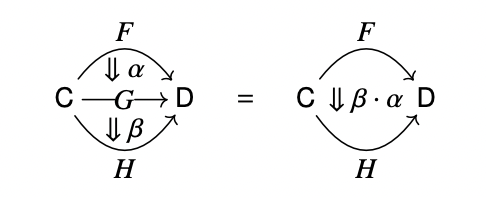
\includegraphics[width=.5\textwidth]{../images/CategoryTheoryInContext/1.png}
\label{}
\end{figure}

There is also a \textbf{horizontal composition} operation
\begin{figure}[htbp]
\centering
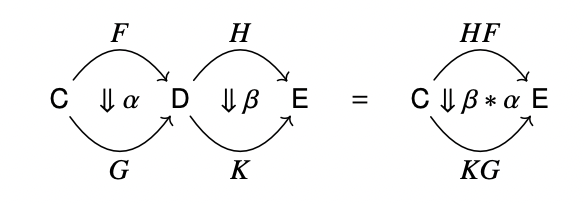
\includegraphics[width=.5\textwidth]{../images/CategoryTheoryInContext/2.png}
\label{}
\end{figure}
defined by the following lemma

\begin{lemma}[horizontal composition]
\label{1.7.4}
Given a pair of natural transformations
\begin{figure}[htbp]
\centering
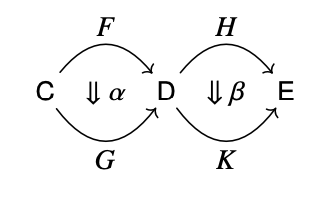
\includegraphics[width=.4\textwidth]{../images/CategoryTheoryInContext/3.png}
\label{}
\end{figure}
there is a natural transformation \(\beta*\alpha:HF\Rightarrow KG\) whose component at \(c\in C\) is defined as the
composite of the following commutative square
\begin{center}\begin{tikzcd}
HFc\ar[r,"\beta_{F_c}"]\ar[rd,dashed,"(\beta*\alpha)_c" description]\ar[d,"H\alpha_c"']
&KFc\ar[d,"K\alpha_c"]\\
HGc\ar[r,"\beta_{G_c}"']&KGc
\end{tikzcd}\end{center}
\end{lemma}

\begin{proof}
\begin{figure}[htbp]
\centering
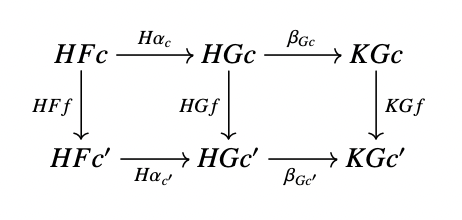
\includegraphics[width=.5\textwidth]{../images/CategoryTheoryInContext/4.png}
\label{}
\end{figure}
\end{proof}

\begin{lemma}[middle four interchange]
Given functors and natural transformations
\begin{figure}[htbp]
\centering
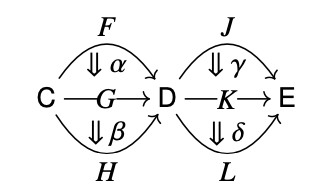
\includegraphics[width=.3\textwidth]{../images/CategoryTheoryInContext/5.png}
\label{}
\end{figure}

the natural transformation \(JF\Rightarrow LH\) defined by first composing vertically and then composing
horizontally equals the natural transformation defined by first composing horizontally and then
composing vertically
\begin{figure}[htbp]
\centering
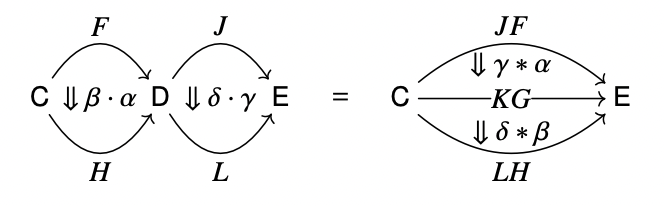
\includegraphics[width=.6\textwidth]{../images/CategoryTheoryInContext/6.png}
\label{}
\end{figure}
\end{lemma}

\begin{definition}[]
A \textbf{2-category} is comprised of
\begin{itemize}
\item objects, e.g., the categories \(\bC\)
\item 1-morphisms between pairs of objects, e.g., the functors \(\bC\xrightarrow{F}\bD\)
\item 2-morphisms between parallel pairs of 1-morphisms, e.g., the natural transformations
\end{itemize}

so that
\begin{itemize}
\item the objects and 1-morphisms form a category, with identities \(1_{\bC}:\bC\to\bC\)
\item For each fixed pair of objects \(\bC\)  and \(\bD\), the 1-morphisms \(F:\bC\to\bD\) and 2-morphisms
between such form a category under an operation called vertical composition
\item There is also a category whose objects are the objects in which a morphism from \(\bC\) to \(\bD\)
is a 2-cell
\begin{equation*}
\nat{\bC}{\bD}{F}{G}{\alpha}
\end{equation*}
\end{itemize}
\end{definition}





\section{{\bfseries\sffamily TODO} CHECK}
\label{sec:org0e660f3}
\ref{1.7.4}
\end{document}
